\section{MATLAB environment}
	As mentioned on chapter \ref{ch:setup}, FLIR software provides as output variables indexed matrices in .mat format, which is MATLAB variable format. Each pixel contains temperature information about itself, it is possible to visualize an example on a scaled image on the following figure:

	\begin{figure}[H]
		\centering
		\captionsetup{justification=centering}
		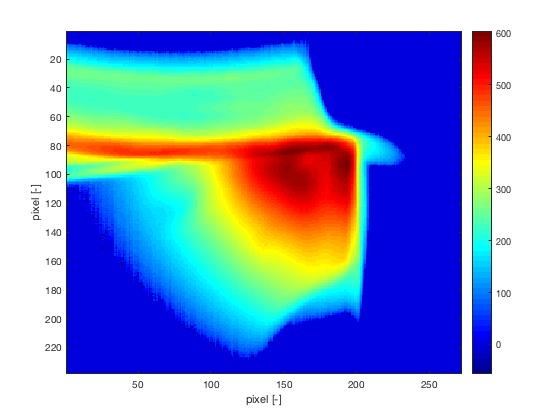
\includegraphics[scale=0.6]{Cap4/TempDist.jpg}
		\caption{Scaled image showing temperature distribution}
		\label{fig:tempdist}
	\end{figure}

	From figure \ref{fig:tempdist} with MATLAB Image Processing Toolbox support it possible to extract much information about the image, such as:

	\begin{itemize}
		\item Edges recognition
		\item Image segmentation for tool, chip and workpiece
		\item Detection of tool tip
		\item Determine isotherms along tool
	\end{itemize}
	
\section{Auxiliar functions}
	\subsection{Contour plot}
	\label{ch:seccontour}
	This is an important tool for this paper, contour plot is able to provide the same level curves. Since the variable used on the process is a temperature matrix, this tool will calculate continuous lines, in which each pixel has a very close temperature measurements. Doing it with a determined and small tolerance, the lines calculated are isotherms of the image. Then, with these lines it is also possible to get its coordinates, which it will be essential to calculate heat carried away from volume control by means of tool.

	\begin{figure}[H]
		\centering
		\captionsetup{justification=centering}
		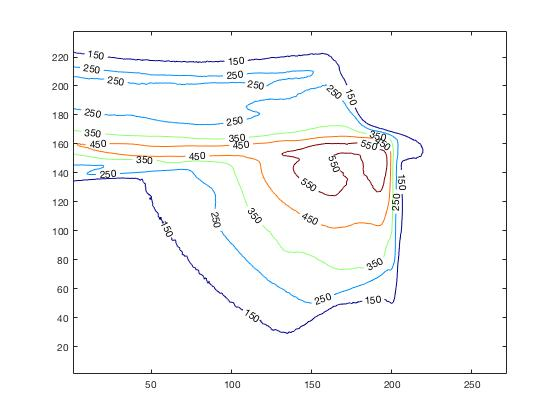
\includegraphics[scale=0.6]{Cap4/contour.jpg}
		\caption{Contour plot}
		\label{fig:contour}
	\end{figure}

	\subsection{Hough lines transformation}
	\label{ch:sechough}
	Hough transform is an extensive method used in computer vision. It is an extraction feature for complex geometries, using normal parameterization for straight lines \cite{duda1972use}. Concerning about the images, the rake and clearance face can be mapped by means of hough lines transformation in MATLAB. It is necessary to provide a probable angle range in what the angular coefficient of sought lines are defined. More precise is this angle range, more reliable and faster will be the output.

	The test bench, where the experiments were held, allows a fixed placement of tool.

	\begin{figure}[H]
		\centering
		\captionsetup{justification=centering}
		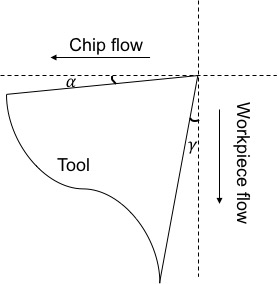
\includegraphics[scale = 0.65]{Cap4/imgset.jpg}
		\caption{Placement of tool}
		\label{fig:imgset}
	\end{figure}

	It means the angle between the rake face and horizontal line and the angle between clearance face and vertical line are always the designed rake and clearance angles, respectively. In other words, the tool does not rotate in relation to the reference axes. Because of this, it is possible to perform hough transformation on the image, being very accurate. As the rake and clearance angle are always $6^{o}$ and $3^{o}$, respectively, the hough transform processing will last a shorter time with predetermined angles than otherwise.

\section{Implementation steps}
	\subsection{Overview}	

	The final aim of the program was able to identify the tool and chip shapes, then the analysis could extract and provide features that were essential for the results of this paper. By means of image processing and some input data, features like maximum cutting zone temperature, maximum chip temperature, heat flows through chip and tool are some examples of what the code is able to provide.	
	\subsection{Finding tool edges}

	As mentioned in the subsection \nameref{ch:sechough}, the method to find tool edges has to provide an accurate range of angles that the rake and clearance angles are inserted. The process is simple and it is demonstrated as follows:

	\lstinputlisting[firstline=223,lastline=257]{ApeA/TemperatureAnalyze.m}

	Since the rake angle is $6^{o}$ and the clearance is $3^{o}$ ranges of [81:85] and [2:5] were given to each respectively, as it is seen on lines 4 and 20. Concerning about the rake angle, the range of angles is given by the complementary angles due to its reference in hough method. In this way, it taken the first 10 highlighted points in the accumulation matrix of hough process, which means the most reasonable points that may represent the edge lines.

	The fixed position of tool allows also the predetermination of the $\rho$ parameter, which is distance of the detected lines from the reference. This is also seen on lines 14 and 30 as boundary conditions to determine the right edge lines. The outputs of this function are the endings coordinates of the detected line and also the angle of the corresponding angular coefficient. 


		\subsubsection{Rake and clearance face}

		With the data provided by the output of hough function, it is possible to extend the lines to match the entire rake and clearance edge. This is an important step of the analysis method because it allows to build an object (binary image) that is a mask to remove only the region of interest, on this case the tool shape. Consequently, it will be possible analyze the temperature fields and thermal behavior in the tool without any interference of the temperatures in the vicinity.

		\begin{figure}[H]
		\centering
		\captionsetup{justification=centering}
		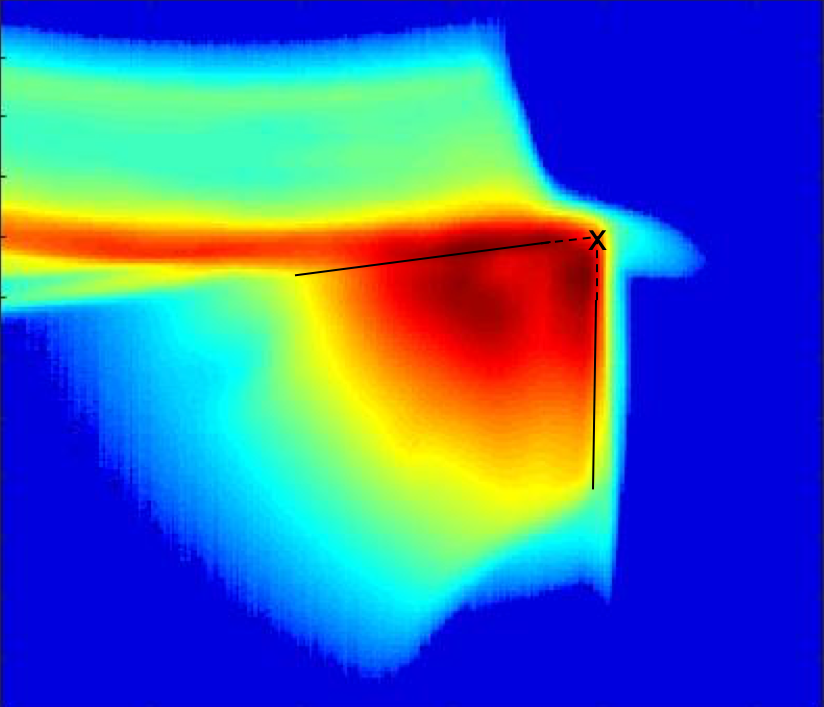
\includegraphics[scale = 0.6]{Imagens/hough.png}
		\caption{Lines detected by hough transformation method}
		\label{fig:hough}
		\end{figure}

		\subsubsection{Tool tip coordinates}

		As the rake and clearance edges are determined, the tool tip will be calculated by means of the intersection between these lines. On the figure \ref{fig:hough} the found lines are extended until they intersect, then the coordinates of tool tip can be calculated. It is important to determine these coordinates due to the interest in knowing the temperatures that the area close to the tip can reach, which is related directly with tool life and therefore the surface finish.

	\subsection{Maximum temperatures}

	As the code were able to segment the tool shape from the entire matrix, it gets easier to extract the other region of interest that present measurable range of temperatures, the chip. Getting the maximum temperature of each zone allows not only to know if the measured temperatures are inside the limit of measurement but also to compare the behavior of this maximum temperature of different cutting velocities and a$_{p}$.

	\subsection{Temperature fields}

	In this step, it will be used the other auxiliary function mentioned on the subsection \nameref{ch:seccontour}. This is an important function to determine same level curves, as the isotherms inside the tool shape. The contour levels are determined in a step of 50 $^{o}$C.

	
	\lstinputlisting[firstline=383,lastline=383]{ApeA/TemperatureAnalyze.m}

	The output of contour function is a matrix C with 2 rows that will provide the levels of temperature and the number of coordinates followed by their absolute values of x and y, which are very valuable when comes to calculate heat flows.

		\begin{mdframed}[backgroundcolor=lightgray!25!]
		\begin{alltt}\fontsize{9pt}{8pt}\fontfamily{pcr}\selectfont
		C    =  [C(1) C(2) C(3) ...C(k)... C(N)]
		C(k) =  [level x(1) x(2)...
		         numxy y(1) y(2)...]
		\end{alltt}
		\end{mdframed}
	
	For each matrix C(k), level shows which temperature it is representing and numxy is the amount of coordinates used to build the level. The coordinates are represented in the pair (x,y).

	\subsection{Heat flows - Chip and Tool}
	\label{heatflows}
	As described on section \ref{methods}, the heat flow through tool and the energy carried away by chip are calculated. For heat flow through the tool, it is possible to extract isothermal lines by means of contour command and to calculate the gradient of temperatures, which already is normal to the isothermal lines due to its properties, with gradient command. The width is already known \ref{sec:exSetup}. The length of the chosen isotherm is done by counting the amount of pixels, provided by the coordinates in contour plot, and turned into millimeter with the scale factor afterwards.
	In the case of the energy carried away by chip, the chosen line is placed on the end of contact chip - tool. The explanation for it is that all the heat source in the friction zone is located before this line, in other words there is no other heat source after this line that could provide more thermal energy to be carried away by chip.		

		\subsubsection{Heat partitions}
		Having the results of the subsection \ref{methods}, these values can be combined with the total power ($P$) generated during the cutting process to calculate the energy that goes to the workpiece by means of energy balance (equation \ref{eq_energybalance}). Then, it is possible to calculate the heat partition relative to each zone of interest.

		\begin{equation} 
		\label{eq_heatpartition}
		p_{i} = \frac{\dot{Q}_{i}}{P}
		\end{equation}

		Which the index i is related to C (chip), W (workpiece) and T (tool).